\documentclass[11pt]{article}

\usepackage{amsmath}
\usepackage{amssymb}
\usepackage{amsfonts}
\usepackage{graphicx}
\usepackage{hyperref}
\usepackage{geometry}
\usepackage{cite}

\geometry{margin=1in}

\title{Dirac-Kaehler Factorization on a Validated Cochain Operator Architecture}
\author{Tomislav Rupi\'c\\Independent Researcher\\\v{S}ibenik, Croatia}
\date{March 2026}

\begin{document}
\maketitle

\begin{abstract}
We study a Dirac-Kaehler lift on the discrete cochain architecture previously used to validate scalar and transverse operator sectors on Gaussian kernel substrates. Earlier work established the scalar Laplacian limit, the edge/Hodge sector, and a low transverse spectral band, while a separate node--spinor Dirac prototype was rejected because its square failed to reproduce the validated scalar operator.

Here we instead construct the graded cochain operator $D_{DK} = d + \delta$ and test its defining square relation against the discrete Hodge Laplacian. On periodic 2D and 3D cochain complexes, the identities $d^2 = 0$, $\delta^2 = 0$, and $D_{DK}^2 = \Delta_H$ hold to numerical precision, including grade-by-grade agreement in 3D. The low graded spectrum is sign-symmetric and remains stable under flat torus-cycle holonomy while preserving the square identity.

These results establish that the validated cochain architecture admits a consistent Dirac-Kaehler lift in 2D and 3D. The interpretation is strictly operator-level: no claim is made regarding fermions, particle content, or quantum field dynamics.
\end{abstract}

\section{Introduction}

Recent work on Gaussian kernel substrates has developed a discrete operator architecture in which multiple sectors are constructed on the same interaction graph rather than introduced independently. The first stage of that program established a kernel-induced scalar operator with a continuum Laplacian limit and identified an edge/Hodge sector supporting a low transverse spectral band with continuum-like scaling. A second stage showed that this transverse sector admits an effective continuum reconstruction and responds in a structured way to controlled scalar deformations of the underlying kernel geometry. Taken together, these results support the view that a single cochain architecture can host multiple operator sectors while remaining numerically tied to the same substrate.

The next structural question is whether this architecture also supports a consistent first-order lift. An earlier node--spinor Dirac-type prototype was tested for this purpose, but it was rejected because its defining square-root criterion failed: although the operator was Hermitian and showed qualitative spectral pairing, its square did not reproduce the validated scalar branch with sufficient accuracy. That failure was informative. It indicated that a directional node--spinor construction was not aligned with the discrete algebra already validated in the cochain framework.

The present work therefore turns to a Dirac--Kaehler construction built directly from the existing discrete exterior calculus on the graph complex. On a graded cochain space, the natural first-order operator is
\[
D_{DK} = d + \delta,
\]
where $d$ is the discrete exterior derivative and $\delta$ is its adjoint under the weighted inner product. The defining algebraic test is therefore the graded identity
\[
D_{DK}^2 = \Delta_H,
\]
with $\Delta_H = d\delta + \delta d$ the discrete Hodge Laplacian. This provides a sharper and more architecture-consistent criterion than the previously rejected node--spinor lift.

The aim of this paper is narrow. We test whether the validated cochain architecture admits a consistent Dirac--Kaehler lift in periodic two- and three-dimensional complexes. The numerical protocol follows the same falsification logic used in earlier stages of the program: first verify the cochain identities, then test the graded square relation, and only after that inspect the low spectrum and its response to flat torus-cycle holonomy. The results show that the square identity holds to numerical precision in both 2D and 3D, including grade-by-grade agreement in 3D, and that the resulting graded spectrum is stable and sign-symmetric under the tested holonomy deformations.

The interpretation remains strictly operator-level. No claim is made here regarding fermions, particle content, or quantum field dynamics. The result is narrower and more concrete: the previously validated cochain architecture supports a consistent discrete Dirac--Kaehler lift.

\section{Cochain Operator Architecture}

The Dirac--Kaehler construction in this work is built on the same discrete cochain architecture used in the earlier scalar and edge-sector studies. The underlying substrate is a periodic cell complex derived from the validated kernel graph construction, with orientation data assigned to cells of each grade. In two dimensions the graded space is
\[
\Omega^0 \oplus \Omega^1 \oplus \Omega^2,
\]
while in three dimensions it becomes
\[
\Omega^0 \oplus \Omega^1 \oplus \Omega^2 \oplus \Omega^3.
\]

Here $\Omega^0$ denotes node-based cochains, $\Omega^1$ oriented edge cochains, $\Omega^2$ oriented face cochains, and $\Omega^3$ oriented volume cochains.

The discrete exterior derivatives are represented by incidence operators between adjacent grades,
\[
d_0 : \Omega^0 \to \Omega^1,
\qquad
d_1 : \Omega^1 \to \Omega^2,
\]
and, in three dimensions,
\[
d_2 : \Omega^2 \to \Omega^3.
\]

Their defining nilpotency relations are

\[
d_1 d_0 = 0
\]

and in three dimensions additionally

\[
d_2 d_1 = 0.
\]

The codifferentials are defined as adjoints

\[
\delta_1 = d_0^{*},\qquad
\delta_2 = d_1^{*},\qquad
\delta_3 = d_2^{*}.
\]

The discrete Hodge Laplacian acts grade by grade as

\[
\Delta_H = d\delta + \delta d .
\]

In the 2D prototype this means
\[
\Delta_H = \mathrm{diag}(\delta_1 d_0,\; d_0\delta_1 + \delta_2 d_1,\; d_1\delta_2),
\]
while in 3D the graded form is
\[
\Delta_H = \mathrm{diag}(\delta_1 d_0,\; d_0\delta_1 + \delta_2 d_1,\; d_1\delta_2 + \delta_3 d_2,\; d_2\delta_3).
\]

With this graded cochain structure in place, the natural first-order operator to test is the Dirac--Kaehler combination $D_{DK} = d + \delta$.

\section{Dirac--Kaehler Lift}
The Stage 6--7 lift is defined directly on the graded cochain space by
\[
D_{DK} = d + \delta,
\]
where $d$ is the block exterior derivative and $\delta$ is the block codifferential assembled from the validated incidence structure and weighted adjoints. On the periodic 2D complex, $D_{DK}$ acts on $\Omega^0 \oplus \Omega^1 \oplus \Omega^2$; on the periodic 3D complex, it acts on $\Omega^0 \oplus \Omega^1 \oplus \Omega^2 \oplus \Omega^3$.

The validation criterion is purely algebraic. The lift is accepted only if its square reproduces the graded Hodge Laplacian to numerical precision,
\[
D_{DK}^2 = \Delta_H,
\]
with agreement required block by block on every grade. This criterion is stricter and more informative than qualitative spectral diagnostics alone. The Stage 5 node--spinor prototype was rejected precisely because its square did not reproduce the validated scalar operator with sufficient accuracy. By contrast, the Dirac--Kaehler construction is designed to live on the same cochain architecture that already validates the scalar and transverse sectors.

\section{Numerical Protocol}
The numerical protocol follows the same falsification sequence in both dimensions:
\begin{itemize}
\item verification of the cochain identities; in 2D this means checking $d_1 d_0 = 0$ and $\delta_1 \delta_2 = 0$, while in 3D the additional checks are $d_2 d_1 = 0$ and $\delta_2 \delta_3 = 0$,
\item graded square test $D_{DK}^2 = \Delta_H$, measured through the global residual and the blockwise residual on each grade,
\item graded spectral diagnostics, including sign pairing, low-mode degeneracy, inverse participation ratio, and the distribution of mode weight across cochain grades,
\item flat-holonomy response, implemented by inserting cycle phases through the periodic identifications and tracking the low spectral flow together with the square residual.
\end{itemize}
All numerical datasets correspond to stamped artifacts committed in the public repository, and the figures below reference those timestamped outputs directly.

\section{Two-Dimensional Prototype (Stage 6)}
The 2D prototype uses periodic square cell complexes at $n = 8, 12, 16$. The cochain identities hold exactly on all tested sizes: the recorded residuals for $d_1 d_0$ and $\delta_1 \delta_2$ are zero, and the graded square residual is also zero on the same runs. The square test then compares $D_{DK}^2$ and $\Delta_H$ spectrally. The mean relative eigenvalue error stays small, at $4.78 \times 10^{-3}$ for $n=8$, $9.92 \times 10^{-3}$ for $n=12$, and $9.28 \times 10^{-3}$ for $n=16$, with blockwise errors reported as zero on all three grades.

The low graded spectrum is sign-symmetric and stable. At $n=12$ the pairing error is $5.38 \times 10^{-3}$, the lowest absolute eigenvalue is $1.09 \times 10^{-17}$, the mean inverse participation ratio is $3.70 \times 10^{-3}$, and the mode weights remain distributed across $\Omega^0$, $\Omega^1$, and $\Omega^2$ rather than collapsing to a single grade. Under flat torus-cycle holonomy, the square residual stays zero and the first positive mode shifts smoothly from $0.51316$ at zero phase to $0.02163$, $0.04325$, and $0.06487$ across the tested cycle phases.

These diagnostics are sufficient for the 2D validation claim: the graded Dirac--Kaehler lift is numerically consistent with the validated 2D cochain architecture and preserves its defining square identity under the tested flat holonomy deformation.

\begin{figure}[t]
\centering
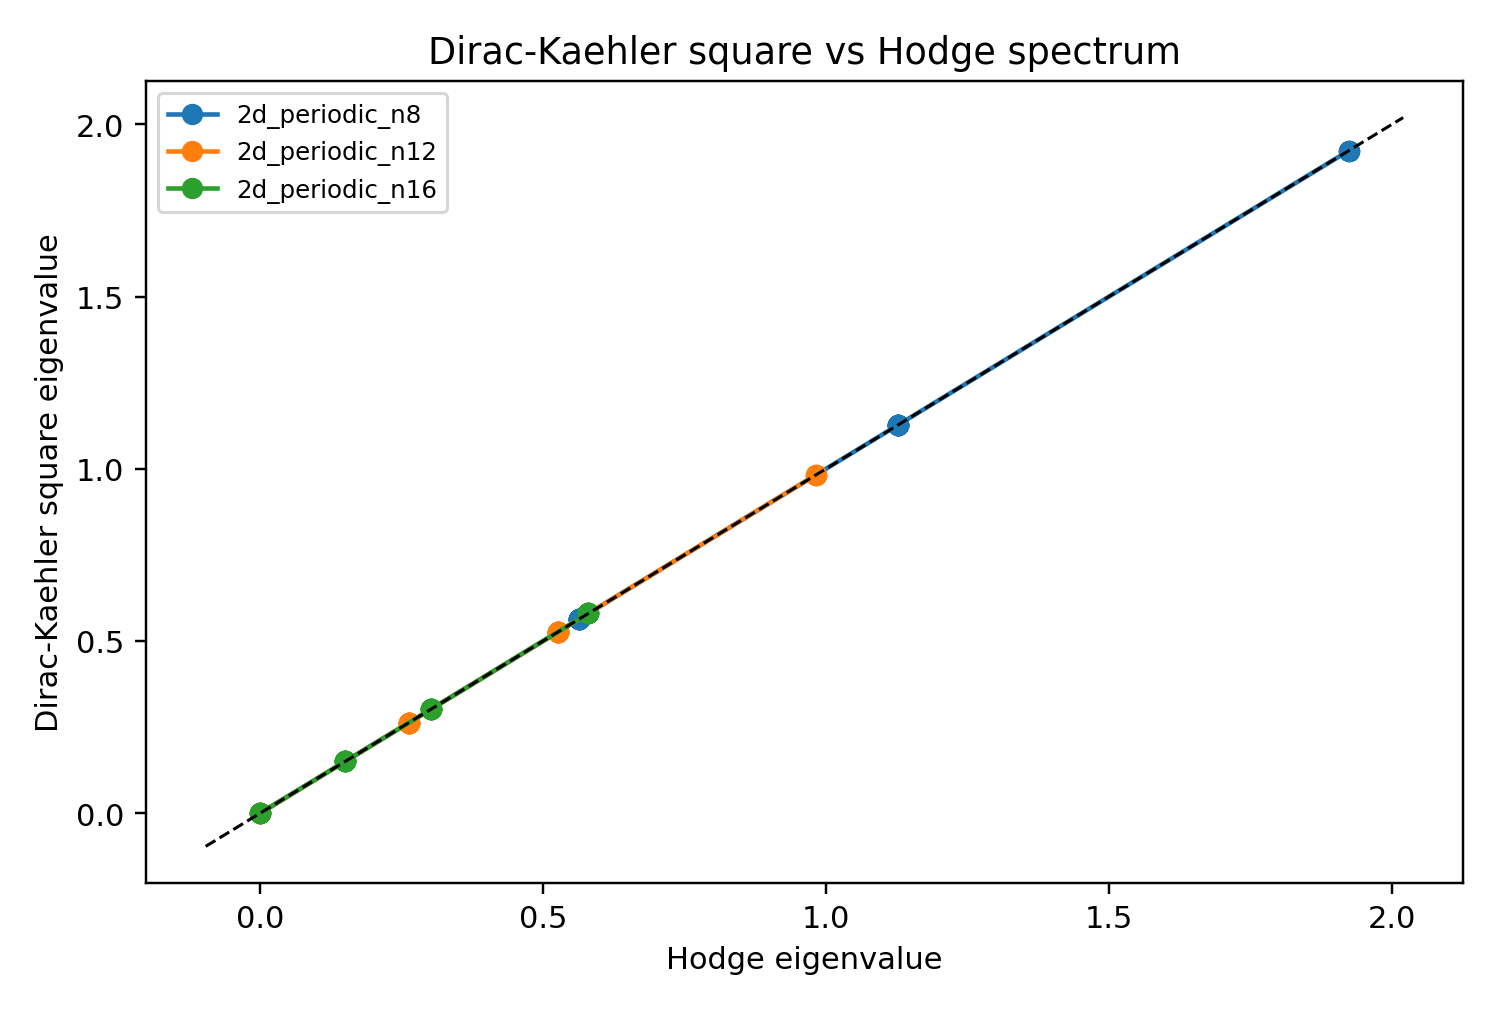
\includegraphics[width=0.48\linewidth]{../plots/20260310_175001_DK_square_vs_Hodge.png}
\hfill
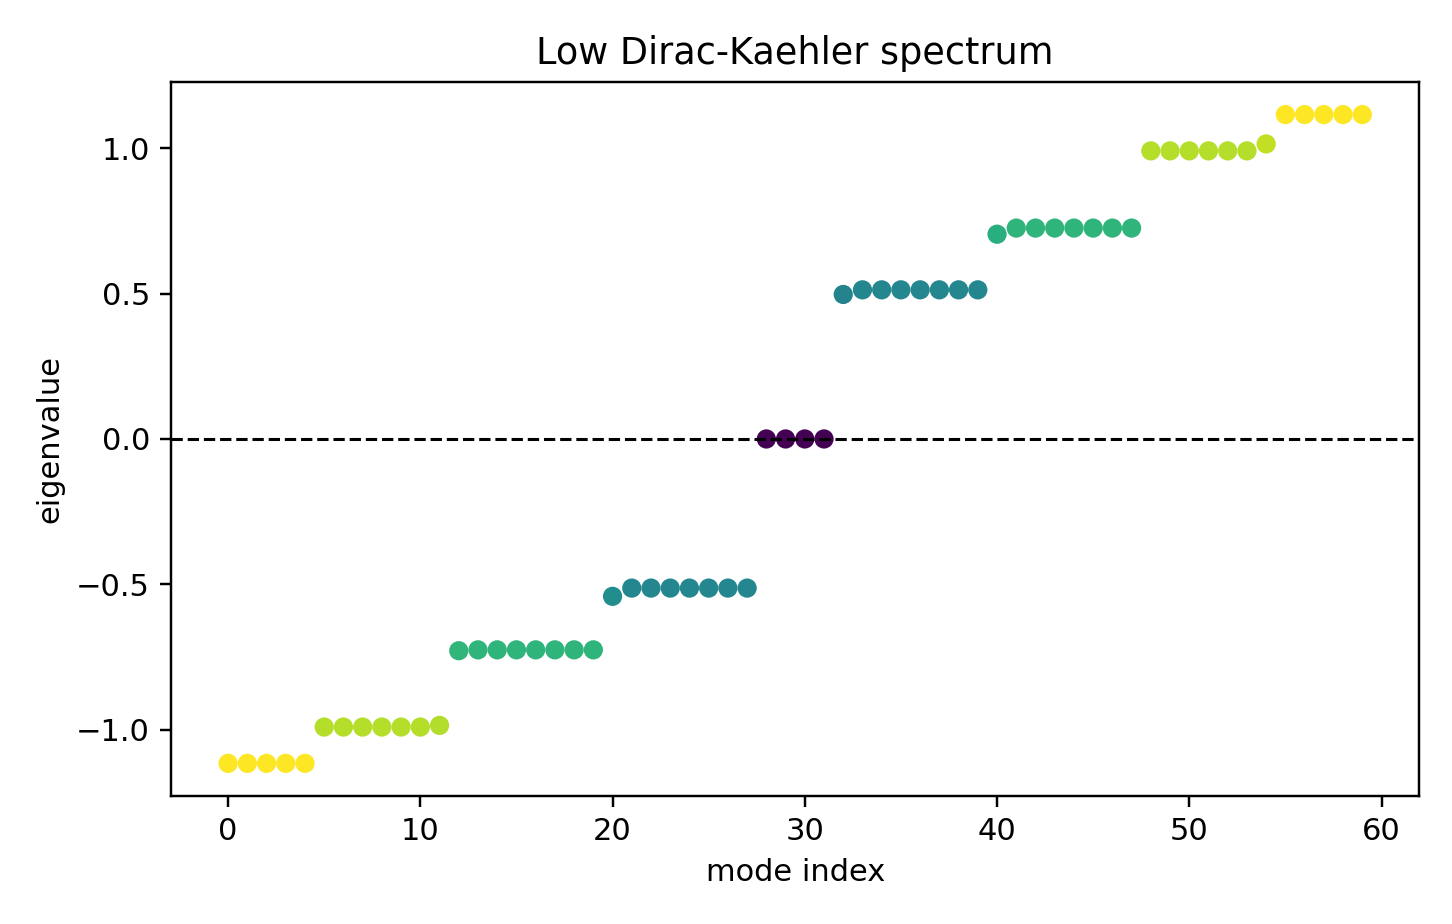
\includegraphics[width=0.48\linewidth]{../plots/20260310_175158_DK_spectrum.png}
\caption{Stage 6 2D prototype. Left: comparison of the low spectrum of $D_{DK}^2$ and $\Delta_H$ for the stamped square test. Right: low graded spectrum of $D_{DK}$ at $n=12$, showing sign symmetry and a near-zero central sector.}
\label{fig:dk2d-square-spectrum}
\end{figure}

\begin{figure}[t]
\centering
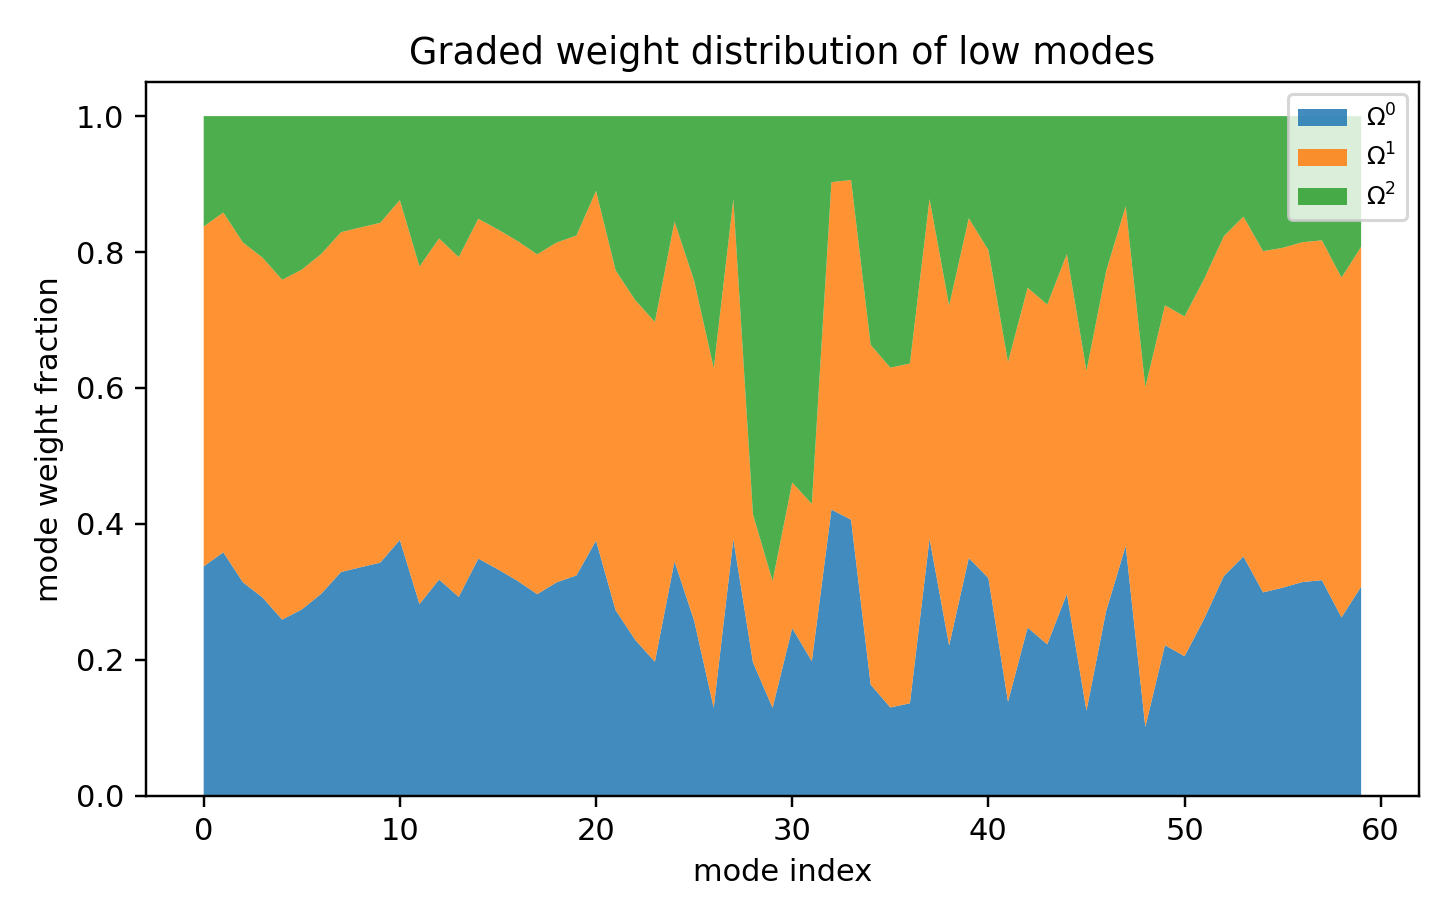
\includegraphics[width=0.48\linewidth]{../plots/20260310_175158_DK_mode_grading.png}
\hfill
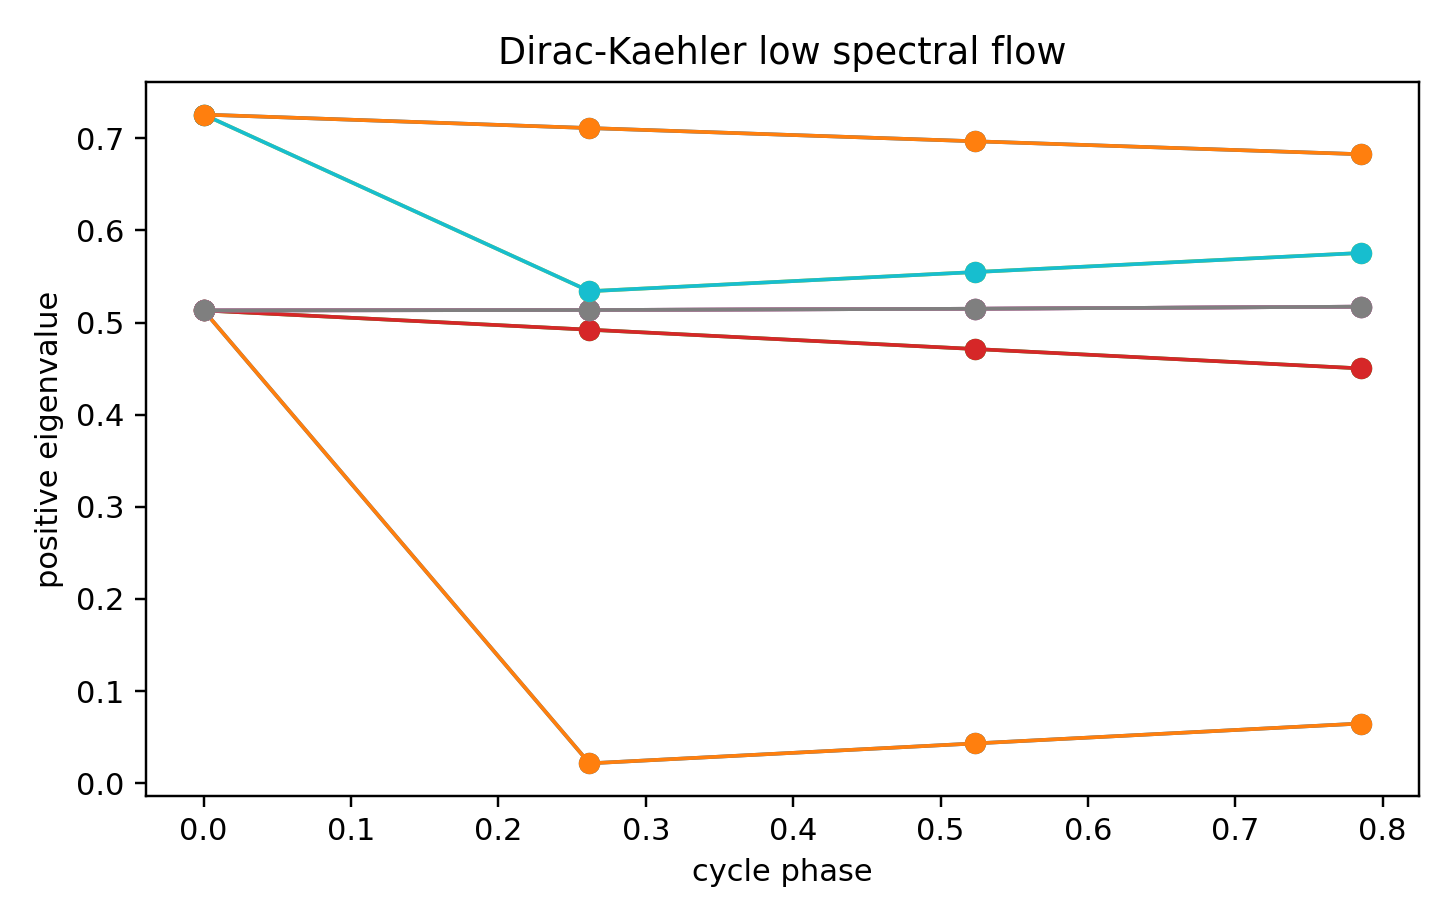
\includegraphics[width=0.48\linewidth]{../plots/20260310_175351_DK_flux_spectral_flow.png}
\caption{Stage 6 2D prototype diagnostics. Left: grade weights of the low modes across $\Omega^0$, $\Omega^1$, and $\Omega^2$. Right: spectral flow of the low positive branch under flat torus-cycle holonomy, with the square identity preserved throughout.}
\label{fig:dk2d-grading-flux}
\end{figure}

\section{Three-Dimensional Extension (Stage 7)}
The 3D extension uses periodic cubic cochain complexes at $n = 4, 6, 8$. This stage was gated by the grade-by-grade square identity. The cochain identities pass exactly: the recorded residuals for $d_1 d_0$, $d_2 d_1$, $\delta_1 \delta_2$, and $\delta_2 \delta_3$ are all zero. The graded square test then gives global relative residuals of $1.39 \times 10^{-16}$ for $n=4$ and zero for $n=6$ and $n=8$. The blockwise relative errors are zero or at numerical roundoff on every grade,
\[
\Omega^0,\; \Omega^1,\; \Omega^2,\; \Omega^3.
\]
The decisive diagnostic is the grade-by-grade residual of $D_{DK}^2 - \Delta_H$, which remains at machine precision across all tested lattice sizes.
This is the decisive Stage 7 pass.

After the gate passed, the low graded spectrum was inspected at $n=6$. The pairing error is $4.75 \times 10^{-4}$, the lowest absolute eigenvalue is $1.64 \times 10^{-19}$, the mean inverse participation ratio is $1.11 \times 10^{-3}$, and the maximum inverse participation ratio is $1.36 \times 10^{-3}$. The low modes remain sign-symmetric and show stable weight distribution across all four grades. Under flat $x$-cycle holonomy at $n=4$, the square residual remains fixed at $1.39 \times 10^{-16}$ while the first positive mode shifts smoothly from $1.30793$ at zero phase to $0.06052$, $0.12098$, and $0.18130$ across the tested cycle phases.

The narrow conclusion is therefore stronger in 3D than in 2D: not only does the graded Dirac--Kaehler operator exist on the periodic cubic cochain complex, but its defining algebraic identity holds grade by grade to numerical precision, and that identity survives the tested flat holonomy deformation.

\begin{figure}[t]
\centering
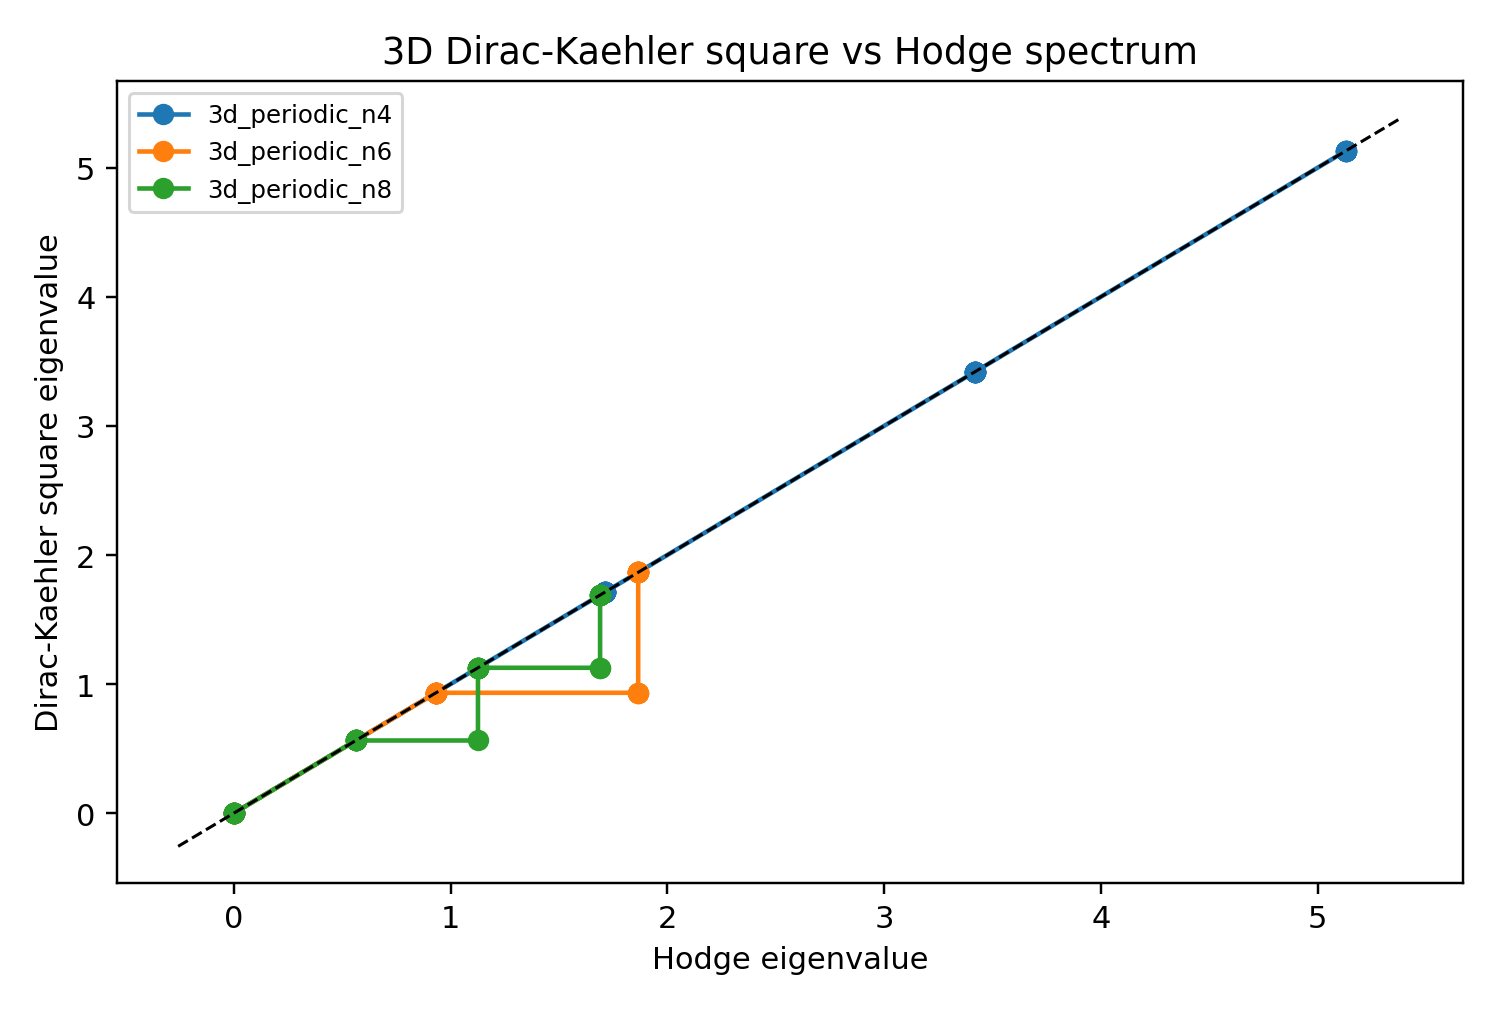
\includegraphics[width=0.48\linewidth]{../plots/20260310_180419_DK_3D_square_vs_Hodge.png}
\hfill
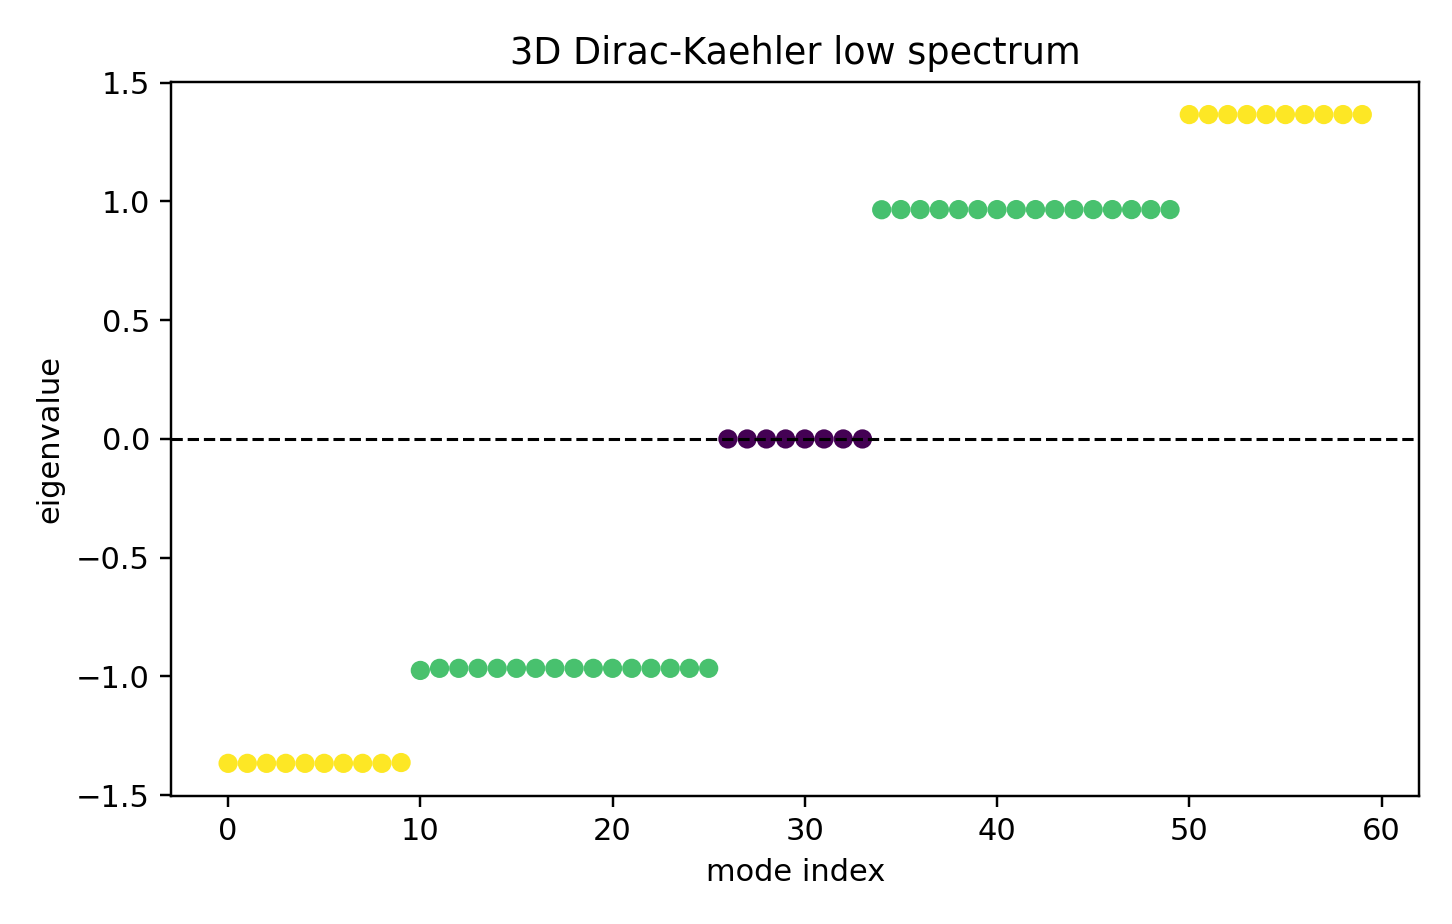
\includegraphics[width=0.48\linewidth]{../plots/20260310_180433_DK_3D_spectrum.png}
\caption{Stage 7 3D extension. Left: comparison of the low spectrum of $D_{DK}^2$ and $\Delta_H$ for the graded square test. Right: low graded spectrum of the 3D Dirac--Kaehler operator at $n=6$, showing stable sign symmetry.}
\label{fig:dk3d-square-spectrum}
\end{figure}

\begin{figure}[t]
\centering
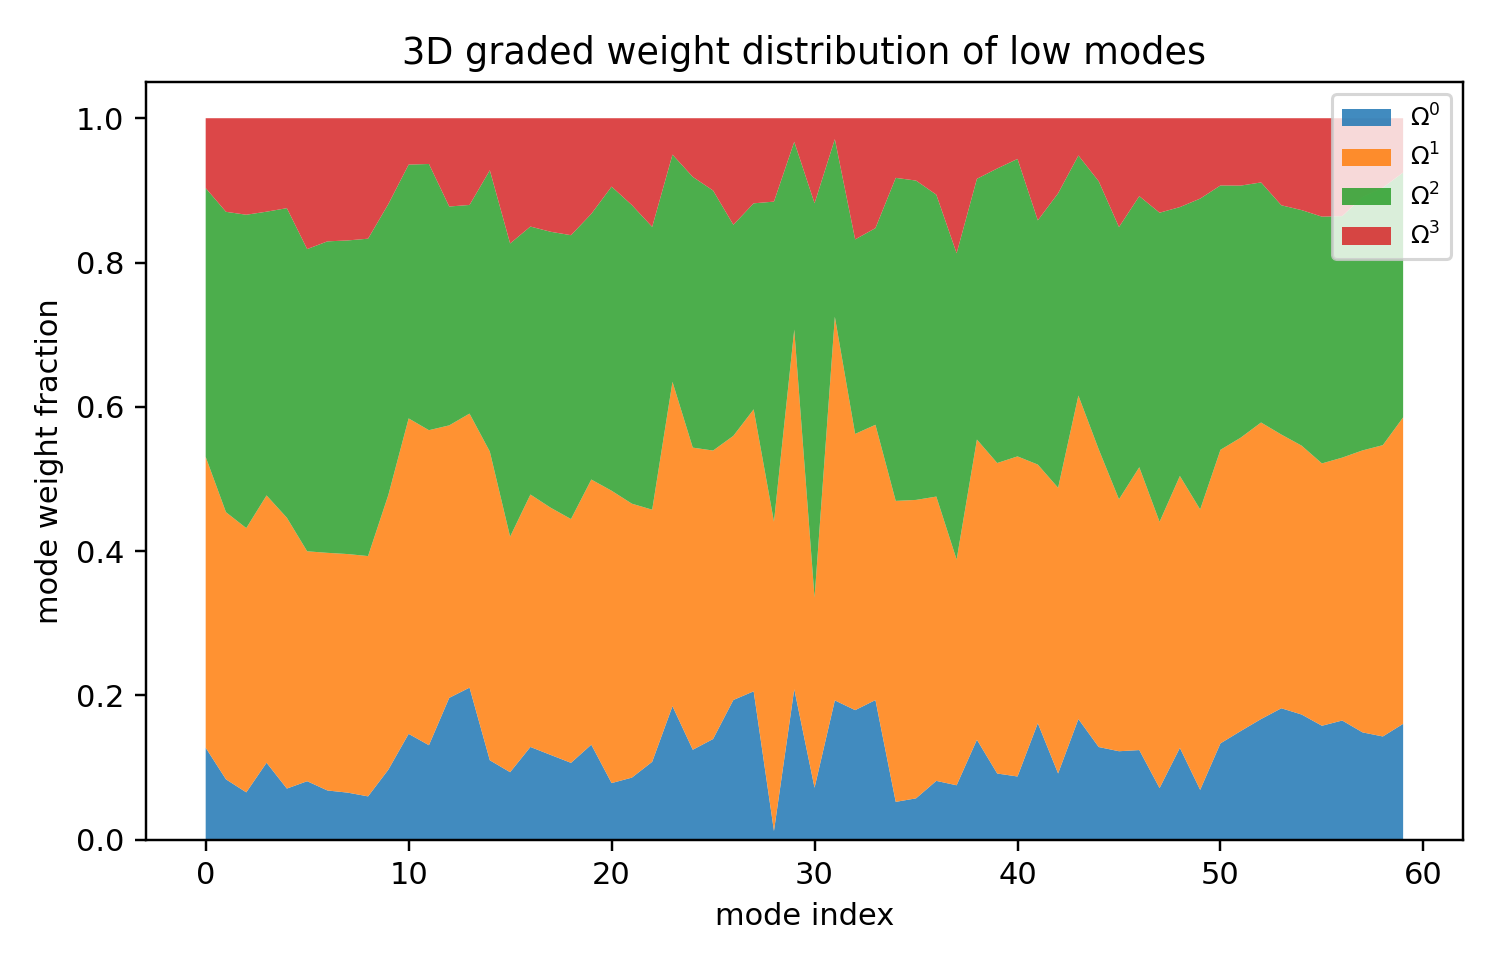
\includegraphics[width=0.32\linewidth]{../plots/20260310_180433_DK_3D_mode_grading.png}
\hfill
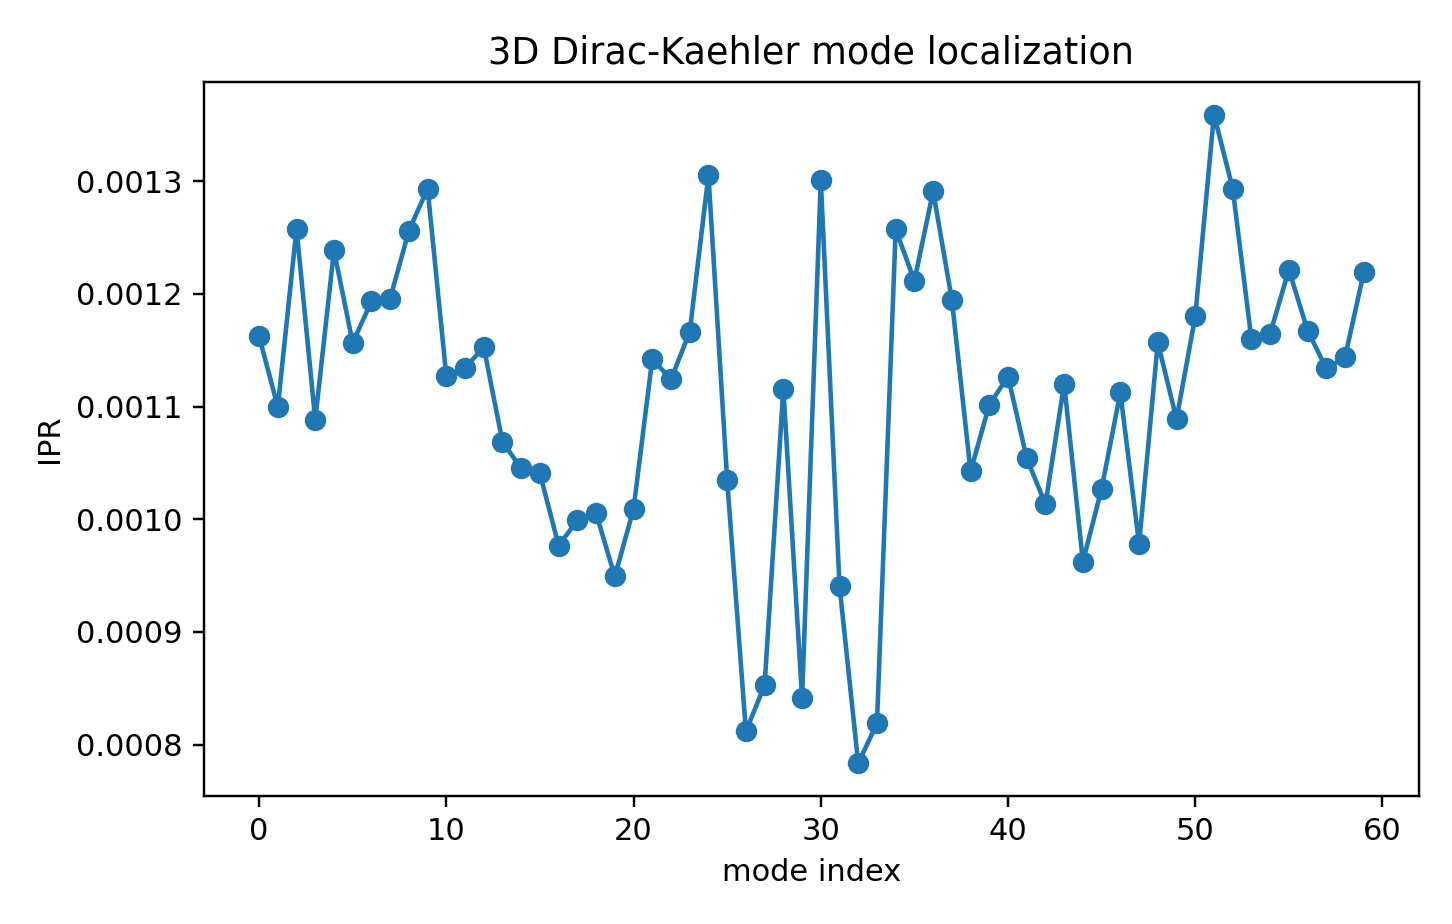
\includegraphics[width=0.32\linewidth]{../plots/20260310_180433_DK_3D_ipr_vs_mode.png}
\hfill
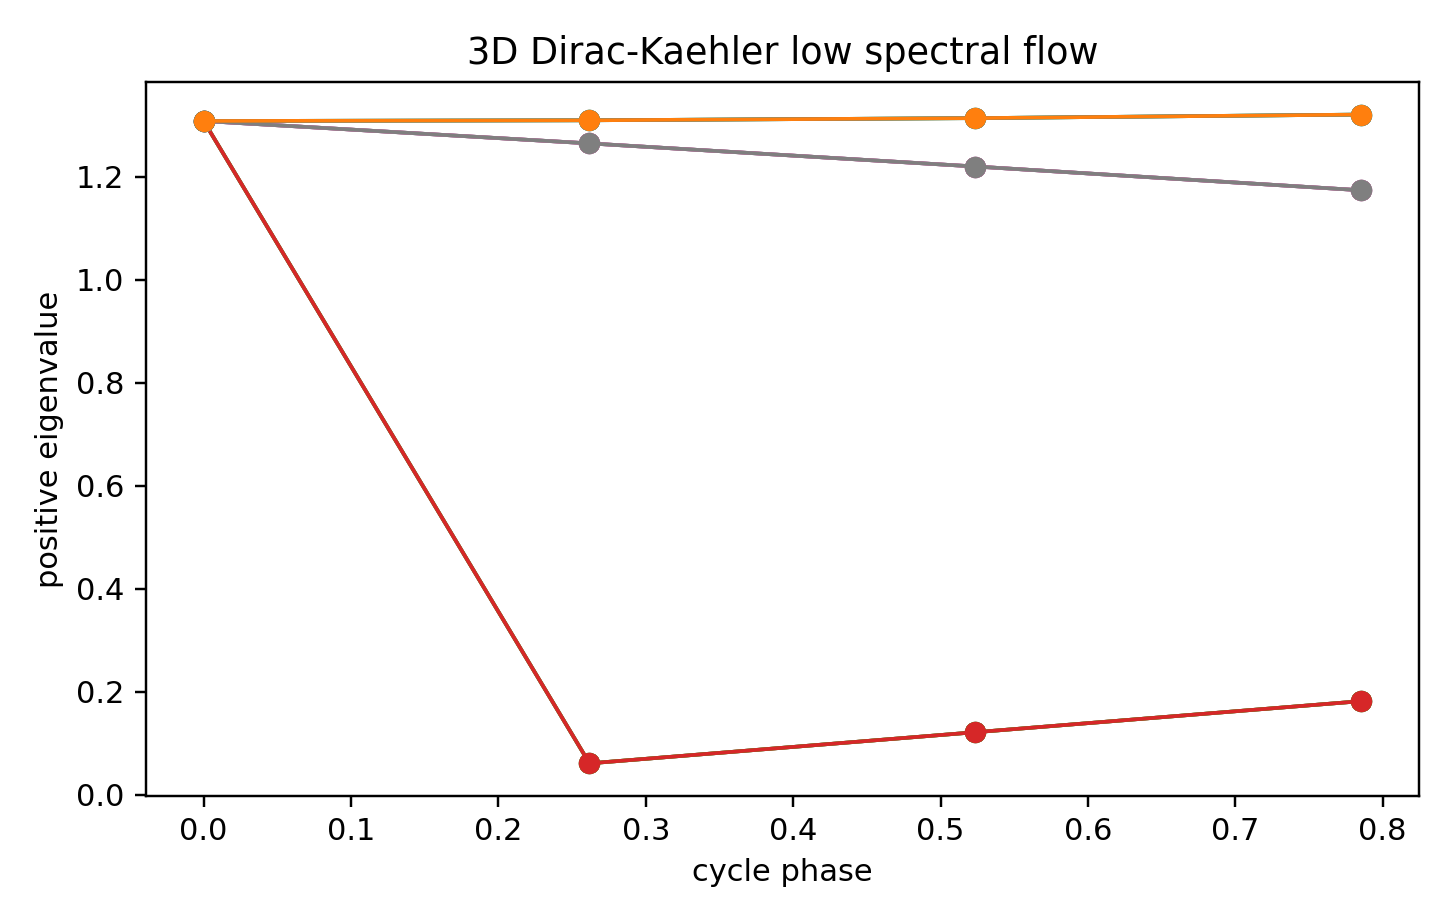
\includegraphics[width=0.32\linewidth]{../plots/20260310_180436_DK_3D_flux_spectral_flow.png}
\caption{Stage 7 3D diagnostics. Left: grade weights of the low modes across $\Omega^0$, $\Omega^1$, $\Omega^2$, and $\Omega^3$. Center: inverse participation ratio versus mode index. Right: low positive spectral flow under flat $x$-cycle holonomy, with the square identity preserved.}
\label{fig:dk3d-grading-flux}
\end{figure}

\section{Interpretation Boundary}
The results reported here are operator-level only. What is established is a discrete algebraic fact on the validated cochain architecture: the graded Dirac--Kaehler operator $D_{DK} = d + \delta$ exists consistently in the tested 2D and 3D periodic complexes, and its square reproduces the graded Hodge Laplacian to numerical precision, including grade-by-grade agreement in 3D.

The paper does not claim fermions, particle content, quantum field theory, or emergent matter. The spectral pairing and holonomy response are reported as properties of the graded discrete operator alone. No physical interpretation beyond that operator-level statement is made.

\section{Conclusion}
This paper documents the next computational milestone in the same kernel-induced operator program. Earlier stages validated the scalar Laplacian limit, the edge/Hodge sector, and a low transverse spectral band, and they also rejected a node--spinor Dirac attempt whose square failed to reproduce the validated scalar branch. The present work instead constructs the Dirac--Kaehler lift directly on the cochain architecture already validated by those stages.

The numerical result is clear. In 2D, the cochain identities hold, the square identity $D_{DK}^2 = \Delta_H$ is satisfied to numerical precision, and the low graded spectrum is stable under flat cycle holonomy. In 3D, the same construction extends to the full graded complex $\Omega^0 \oplus \Omega^1 \oplus \Omega^2 \oplus \Omega^3$, and the square identity holds grade by grade to numerical precision on the tested periodic cochain complexes.

The narrow conclusion is therefore that the validated cochain architecture supports a consistent Dirac--Kaehler lift in 2D and 3D. This is a structural operator result only. Future work may refine the 3D graded continuum comparison, test larger lattices, and examine how the Dirac--Kaehler lift interacts with the previously validated scalar and transverse sectors.

\begin{thebibliography}{9}

\bibitem{paper1}
Tomislav Rupi\'c,
\newblock \emph{Kernel-Induced Operator Architecture and the Emergence of a Transverse Spectral Band on Discrete Substrates},
\newblock HAOS-IIP preprint, 2026.

\bibitem{paper2}
Tomislav Rupi\'c,
\newblock \emph{Continuum Reconstruction and Scalar-Transverse Coupling in Kernel-Induced Operator Systems},
\newblock HAOS-IIP preprint, 2026.

\bibitem{repo}
Tomislav Rupi\'c,
\newblock \emph{HAOS-IIP Repository and Stamped Numerical Artifacts},
\newblock GitHub repository, \url{https://github.com/tomislavrupic}.

\end{thebibliography}

\end{document}
